\section{Potential flow}
\subsection{The continuity equation for incompressible flow}
The idealised fluid in this essay is incompressible. This means that if $\rho$ represents the density of the fluid, then as per definition \ref{definition:INCOMPRESSIBLE}, $\rho$ must 
remain constant over time at every point in the domain of the vector field representing the fluid flow. This means that for any arbitrary closed volume within the fluid, the net mass
flow rate across its boundaries must be zero.

Let the velocity vector field of the fluid be $\mathbf{V}:x,y\mapsto X(x,y)\ihat+Y(x,y)\jhat$. To quantify the mass flow, consider an arbitrary infinitesimal rectangular volume within
the fluid, with vertices $W(\alpha_0,\beta_0)$, $X(\alpha_1,\beta_0)$, $Y(\alpha_1,\beta_1)$, and $Z(\alpha_0,\beta_1)$, as depicted below. Let $\bar{\alpha}=\frac{\alpha_0+\alpha_1}{2}$
and $\bar{\beta}=\frac{\beta_0+\beta_1}{2}$. Assume $\mathbf{V}$ is continuous and differentiable over this region.

\begin{center}
    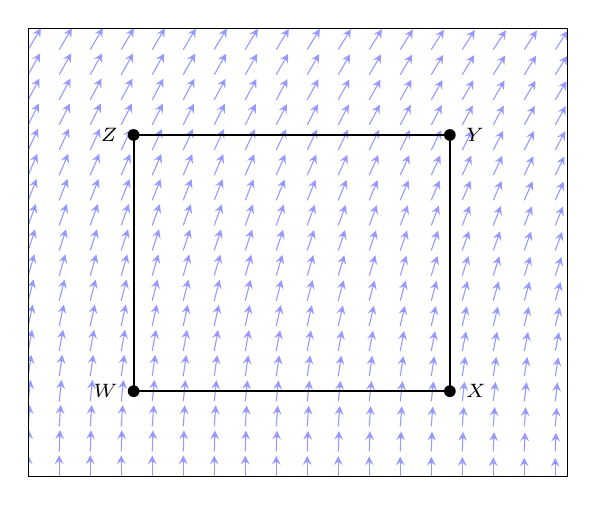
\begin{tikzpicture}[scale=1,X/.style = {circle, fill=black, inner sep=1.5pt,
            label={[font=\scriptsize]left:#1},
            node contents={}},Y/.style = {circle, fill=black, inner sep=1.5pt,
            label={[font=\scriptsize]right:#1},
            node contents={}}]
        \begin{axis}
        [
            domain=0:0.5,
            view={0}{90},
            xtick=\empty,
            ytick=\empty
        ]
        \addplot3[blue, opacity=0.4, quiver={u={sin(deg(y))}, v={cos(deg(x))}, scale arrows=0.025}, -stealth,samples=18] {0};
        \draw[draw=black, thick] (0.1,0.1) rectangle ++(0.3,0.3);
        \draw (0.1,0.1) node[X={$W$}];
        \draw (0.4,0.1) node[Y={$X$}];
        \draw (0.4,0.4) node[Y={$Y$}];
        \draw (0.1,0.4) node[X={$Z$}];
        \end{axis}
    \end{tikzpicture}
\end{center}

The mass flow rate ($\dot{m}$, mass per unit time) across a given surface is defined as the flux of mass, which is computed as the product of density, the velocity component normal to the
surface, and the area of the surface. Thus along the $x$ axis (in the direction of $\ihat$) the mass flow rate into $WZ$ is given as,
$$
    \dot{m}_{\rightarrow WZ}=\rho X(\alpha_0,\bar{\beta})(\beta_1-\beta_0)
$$
and similarly the mass flow rate out of the opposite side $XY$ is given as:
$$
    \dot{m}_{XY\rightarrow}=\rho X(\alpha_1,\bar{\beta})(\beta_1-\beta_0)
$$
Thus, the net mass flow rate out of the rectangular region along the $x$ axis is:
\begin{align*}
    \dot{m}_{\ihat}&=\dot{m}_{XY\rightarrow}-\dot{m}_{\rightarrow WZ}\\
    &=\rho X(\alpha_1,\bar{\beta})(\beta_1-\beta_0)-\rho X(\alpha_0,\bar{\beta})(\beta_1-\beta_0)
\end{align*}
Which, factoring out $\rho(\beta_1-\beta_0)$, leads to:
$$
    \dot{m}_{\ihat}=\rho(\beta_1-\beta_0)\left[X(\alpha_1,\bar{\beta})-X(\alpha_0,\bar{\beta})\right]
$$
Analogously, across the $y$ axis, the net mass flow rate out of the rectangular region between sides $WX$ and $ZY$ is given by the expression:
$$
    \dot{m}_{\jhat}=\rho(\alpha_1-\alpha_0)\left[Y(\bar{\alpha},\beta_1)-Y(\bar{\alpha},\beta_0)\right]
$$
Therefore, the net mass flow rate out of the rectangular region, which must be equal to 0 for the fluid to incompressible, is given by:
\begin{align*}
    \dot{m}&=\dot{m}_{\ihat}+\dot{m}_{\jhat}\\
    &=\rho(\beta_1-\beta_0)\left[X(\alpha_1,\bar{\beta})-X(\alpha_0,\bar{\beta})\right]+\rho(\alpha_1-\alpha_0)\left[Y(\bar{\alpha},\beta_1)-Y(\bar{\alpha},\beta_0)\right]=0
\end{align*}
Dividing through by $\rho$, $(\alpha_1-\alpha_0)$ and $(\beta_1-\beta_0)$:
$$
    \frac{X(\alpha_1,\bar{\beta})-X(\alpha_0,\bar{\beta})}{\alpha_1-\alpha_0}+\frac{Y(\bar{\alpha},\beta_1)-Y(\bar{\alpha},\beta_0)}{\beta_1-\beta_0}=0
$$
Now consider the limit as $\alpha_1\rightarrow\alpha_0$ and $\beta_1\rightarrow\beta_0$, the difference $\delta_\alpha=\alpha_1-\alpha_0\rightarrow0$ and $\delta_\beta=\beta_1-\beta_0\rightarrow0$.
\begin{align*}
    \lim_{\delta_\alpha\rightarrow0}\frac{X(\alpha_0+\delta_\alpha,\bar{\beta})-X(\alpha_0,\bar{\beta})}{\delta_\alpha}&=\eval{\pdv{X}{x}}_{\point{\alpha_0}{\bar{\beta}}}\\
    \lim_{\delta_\beta\rightarrow0}\frac{Y(\bar{\alpha},\beta_0+\delta_\beta)-Y(\bar{\alpha},\beta_0)}{\delta_\beta}&=\eval{\pdv{Y}{y}}_{\point{\bar{\alpha}}{\beta_0}}
\end{align*}
Furthermore, as $\alpha_1\rightarrow\alpha_0$ and $\beta_1\rightarrow\beta_0$, $\bar{\alpha}\rightarrow\alpha_0$ and $\bar{\beta}\rightarrow\beta_0$, consequently
$$
    \dot{m}=\eval{\pdv{X}{x}}_{\point{\alpha_0}{\beta_0}}+\eval{\pdv{Y}{y}}_{\point{\alpha_0}{\beta_0}}=\eval{\divergence{\mathbf{V}}}_{\point{\alpha_0}{\beta_0}}=0
$$
Because $\point{\alpha_0}{\beta_0}$ is any point in the domain of $\mathbf{V}$ where the function is differentiable, the expression can be generalised as
$$
    \divergence{\mathbf{V}}=0
$$
This equation is known as the continuity equation for incompressible fluids \cite{PHAM2014405} and will underpin following derivations made in this essay.

\subsection{Irrotational flow}\label{section:IRROTATIONAL}
As mentioned in definition \ref{definition:VP}, one resulting property of the idealisations (steady, inviscid and incompressible flow)
made in this essay is irrotational flow. If flow is rotational, then there exists points at which $\curl{\fatf}\neq0$. In other words, if one were to
imagine a water wheel at some point in the fluid, and it spins, then the flow is rotational, and vice versa for irrotational flow.
However, flow being irrotational does not imply that it cannot curve, for example $\curl{\fatf}=0$ in cases such as:
\begin{align*}
    &\fatf:x,y\mapsto X(x,y)\ihat+Y(x,y)\jhat\quad\forall\point{x}{y}\neq\point{0}{0}\\
    &X:x,y\mapsto-\frac{y}{x^2+y^2}\,,\quad Y:x,y\mapsto\frac{x}{x^2+y^2}
\end{align*}
Applying the quotient rule to compute the derivatives for both $X$ and $Y$ gives:
\begin{align*}
    \pdv{X}{y}&=-\frac{\left(\pdv{y}y\right)\left(x^2+y^2\right)-y\pdv{y}\left(x^2+y^2\right)}{\left(x^2+y^2\right)^2}\\
    &=-\frac{x^2+y^2-y(2y)}{\left(x^2+y^2\right)^2}\\
    &=-\frac{x^2-y^2}{\left(x^2+y^2\right)^2}
\end{align*}
\begin{align*}
    \pdv{Y}{x}&=\frac{\left(\pdv{x}x\right)\left(x^2+y^2\right)-x\pdv{x}\left(x^2+y^2\right)}{\left(x^2+y^2\right)^2}\\
    &=\frac{x^2+y^2-x(2x)}{\left(x^2+y^2\right)^2}\\
    &=\frac{-x^2+y^2}{\left(x^2+y^2\right)^2}=-\frac{x^2-y^2}{\left(x^2+y^2\right)^2}
\end{align*}
Thus,
\begin{align*}
    \pdv{X}{y}=\pdv{Y}{x}\implies\pdv{Y}{x}-\pdv{X}{y}=0\\
    \therefore\curl{\fatf}=0
\end{align*}
Plotting the vector field for $\fatf$ reveals circulation around the origin, suggesting rotational flow, but which, with a curl of 0 (everywhere except for
the origin, where $\fatf$ is undefined), is irrotational\referto{figure}{figure:ZEROCURL}.
\begin{figure*}[!ht]
    \includegraphics[scale=0.5]{0_curl.pdf}
    \centering
    \caption{The function $\fatf:x,y\mapsto\begin{pmatrix}
        -y\left(x^2+y^2\right)^{-1}\\x\left(x^2+y^2\right)^{-1}
    \end{pmatrix}$ is irrotational despite curving}
    \label{figure:ZEROCURL}
\end{figure*}

\subsection{The velocity potential}
The velocity potential $\phi$ of some vector field $\mathbf{V}$ is defined as a scalar field such that:
$$
    \gradient{\phi}=\mathbf{V}
$$
Such a velocity potential exists for all irrotational flow, like the flow modelled in this essay. To prove the existance of the velocity potential, consider the
identity $\curl{\gradient{\varphi}}$, where $\varphi$ is a function of $x$ and $y$ and is scalar valued. $\gradient{\varphi}$ is defined as
$$
    \gradient{\varphi}=\begin{bmatrix}
        \pdv*{\varphi}{x}\\
        \pdv*{\varphi}{y}
    \end{bmatrix}
$$
Taking the curl of this expression and applying Theorem~\ref{lemma:CLAIRAUT} (Clairaut's theorem) gives
\begin{align*}
    \curl{\gradient{\varphi}}&=\pdv{\varphi}{y}{x}-\pdv{\varphi}{x}{y}\\
                             &=\pdv{\varphi}{y}{x}-\pdv{\varphi}{y}{x}=0
\end{align*}

\section{Formulation of the problem}
\section{Governing equations and boundary Conditions}